\documentclass[11pt,a4paper]{article}

\usepackage[utf8]{inputenc}
\usepackage[T1]{fontenc}
\usepackage{lmodern}
\usepackage{microtype}
\usepackage[margin=2.4cm]{geometry}
\usepackage{amsmath,amssymb}
\usepackage{graphicx}
\usepackage{booktabs}
\usepackage{float}
\usepackage{caption}
\usepackage{xcolor}
\usepackage[hidelinks]{hyperref}

\captionsetup{
    font=small,
    labelfont=bf,
    width=0.95\textwidth
}

\title{\textbf{Adjoint-Based Aerodynamic Shape Optimization of the NACA~0012 Airfoil\\
under Pitching-Moment and Geometric Constraints}}
\author{Kacper Piechocki}
\date{}

\begin{document}

\maketitle

\begin{abstract}
This report presents a gradient-based aerodynamic shape optimization of the NACA~0012 airfoil in subsonic turbulent flow ($M = 0.15$, $Re = 3 \times 10^6$, $\alpha = 2.0^\circ$). The optimization framework couples the SU2 discrete-adjoint Reynolds-Averaged Navier--Stokes (RANS) solver with the Method of Moving Asymptotes (MMA) algorithm from NLopt and a 16-variable Free-Form Deformation (FFD) parameterization. The objective is to maximize the lift-to-drag ratio $L/D$ subject to a trim pitching-moment constraint ($|C_{Mz}| \leq 0.05$), local structural thickness preservation ($t/t_0 \geq 0.90$ across nine chordwise stations), and strict leading- and trailing-edge pinning ($|\Delta y_{\mathrm{LE,TE}}| \leq 5\times 10^{-4}c$) to prevent artificial pitch rotation. Discrete-adjoint sensitivities and analytical geometric constraints are verified against central finite differences prior to optimization. Within 16 evaluations, followed by an independent 4500-iteration CFD verification, the optimized airfoil increases $L/D$ from $24.00$ to $45.65$ ($+90.2\%$) while maintaining all aerodynamic and geometric constraints ($C_{Mz} = 0.0496$, $\min(t/t_0) = 0.991$, $\Delta\alpha_{\mathrm{eff}} = +0.05^\circ$). An off-design polar sweep over $\alpha \in [-2^\circ, 10^\circ]$ confirms that the pinned design outperforms the baseline across the entire tested incidence range, raising peak efficiency from $L/D_{\max} = 64.19$ to $70.73$ ($+10.2\%$) and reducing drag by $4$--$11$ counts at matched lift ($C_L \geq 0.65$). A comparative case without edge pinning demonstrates that unpinned optimization achieves a higher apparent efficiency ($L/D = 62.80$) primarily by rotating the chord nose-up by $\Delta\alpha_{\mathrm{eff}} \approx +2.7^\circ$ and introducing a trailing-edge reflex, confirming the methodological importance of explicit edge pinning in single-point shape optimization at fixed angle of attack.
\end{abstract}

\section{Introduction}

Aerodynamic shape optimization (ASO) is a standard tool in modern wing and airfoil design, enabling systematic improvements in aerodynamic efficiency under realistic structural and flight-mechanics constraints. In high-dimensional design spaces, gradient-free methods quickly become computationally prohibitive when coupled with Reynolds-Averaged Navier--Stokes (RANS) flow solvers. Discrete-adjoint methods resolve this bottleneck by computing the gradient of an aerodynamic functional with respect to all design variables at a cost comparable to a single primal flow solution, largely independent of the number of design parameters.

At low angles of attack, symmetric airfoils such as the NACA~0012 operate well below their maximum lift-to-drag ratio. Introducing camber significantly increases lift at a modest drag penalty, but unrestricted optimization at a fixed angle of attack typically exploits two undesirable mechanisms: excessive nose-down pitching moments that increase trim drag, and rigid-body-like rotation of the airfoil chord inside the deformation box that masks an increase in effective angle of attack as a shape improvement.

The objective of this work is to build and validate a fully automated, physically constrained adjoint optimization pipeline using SU2 (Release~8.5.0) and NLopt. Specifically, the study addresses five elements:
\begin{enumerate}
    \item Formulation of a constrained $L/D$-maximization problem combining a single quotient-rule discrete adjoint for $C_D/C_L$, a second discrete adjoint for $C_{Mz}$, and analytical Bernstein-polynomial constraints for thickness and edge pinning.
    \item Verification of both geometric and adjoint derivatives against central finite differences.
    \item Execution of the optimization loop with continuous flow warm-starting, followed by independent high-iteration CFD verification.
    \item Quantitative comparison between unpinned and pinned leading-/trailing-edge formulations to decouple pure camber optimization from effective pitch rotation.
    \item Off-design polar evaluation over $\alpha \in [-2^\circ, 10^\circ]$ to assess aerodynamic robustness and trim behavior away from the design point.
\end{enumerate}

\section{Numerical Methodology}

\subsection{Flow Conditions and Governing Equations}

The aerodynamic analysis solves the two-dimensional steady compressible RANS equations using the finite-volume solver \texttt{SU2\_CFD}. The design point corresponds to low-subsonic turbulent flow over a unit-chord airfoil ($c = 1.0$) with the freestream and numerical parameters summarized in Table~\ref{tab:solver_setup}.

\begin{table}[H]
\centering
\caption{Freestream conditions and numerical discretization settings used in SU2.}
\label{tab:solver_setup}
\begin{tabular}{ll}
\toprule
Parameter & Value / Setting \\
\midrule
Mach number, $M$ & $0.15$ \\
Reynolds number, $Re$ & $3.0 \times 10^6$ \\
Angle of attack, $\alpha$ & $2.0^\circ$ \\
Freestream temperature, $T_\infty$ & $288.15\text{ K}$ \\
Moment reference point & $(x/c, y/c) = (0.25, 0.0)$ \\
Turbulence model & Menter $k$--$\omega$ SST-2003m (fully turbulent, no transition) \\
Freestream turbulence & $TI = 0.1\%$, $\mu_t / \mu_l = 10.0$ \\
Convective flux (flow / turb.) & Roe (2nd-order MUSCL, no limiter) / Scalar Upwind \\
Gradient reconstruction & Weighted Least Squares \\
Time integration & Euler Implicit, ILU(0) preconditioning (tol. $10^{-6}$) \\
Primal CFL strategy & Adaptive CFL ($10.0 \to [10.0, 100.0]$) \\
Adjoint solver & Discrete adjoint (\texttt{SU2\_CFD\_AD}), fixed $\mathrm{CFL} = 50.0$, frozen limiter \\
\bottomrule
\end{tabular}
\end{table}

Two deliberate modeling choices were made to ensure smooth gradients and robust discrete-adjoint convergence. First, laminar-turbulent transition modeling was disabled (\texttt{KIND\_TRANS\_MODEL = NONE}) so that the optimization operates in a smooth, fully turbulent regime. Second, the convective slope limiter was deactivated (\texttt{SLOPE\_LIMITER\_FLOW = NONE}), which is well suited for shock-free subsonic flow ($M = 0.15$) and improved primal density residual convergence by roughly two orders of magnitude relative to a Venkatakrishnan-limited scheme.
Following the default right-handed SU2 coordinate convention ($+x$ streamwise, $+y$ upward, $+z$ out of the page), pitching moments about the quarter-chord $(0.25c, 0)$ are positive nose-down ($C_{Mz} > 0$), opposite to the classical stability-axis sign convention ($C_m < 0$ nose-down).
\subsection{Computational Mesh and Deformation}

The computational domain is discretized with a hybrid unstructured 2D grid generated in Gmsh and previously validated against the NASA reference NACA~0012 grid (\texttt{n0012\_897-257.su2}) in an accompanying aerodynamic characterization study. The far-field boundary is a circle of radius $R = 15c$ centered at $(0.5, 0)$. The trailing edge is closed with a convex circular arc discretized by 20 transfinite nodes to avoid a singular sharp corner.

The mesh exported to SU2 comprises $187{,}863$ grid points and $252{,}122$ two-dimensional elements, consisting of $121{,}481$ structured quadrilateral cells in the boundary layer and $130{,}641$ background triangles, with $2{,}059$ boundary edges on the airfoil surface and $64$ on the far-field boundary. The boundary layer starts with a first-cell height of $10^{-5}c$ and grows at a ratio of $1.10$ up to a thickness of $0.03c$, while a refinement box ($x/c \in [0.9, 1.5]$, $y/c \in [-0.15, 0.15]$) resolves the near wake. Element quality measured by the Gmsh $\mathrm{minSICN}$ metric averages $0.7186$, with a minimum value of $0.0200$ in the highest-aspect-ratio boundary-layer transitions. Key regions of the mesh topology are shown in Figure~\ref{fig:mesh}.

\begin{figure}[H]
    \centering
    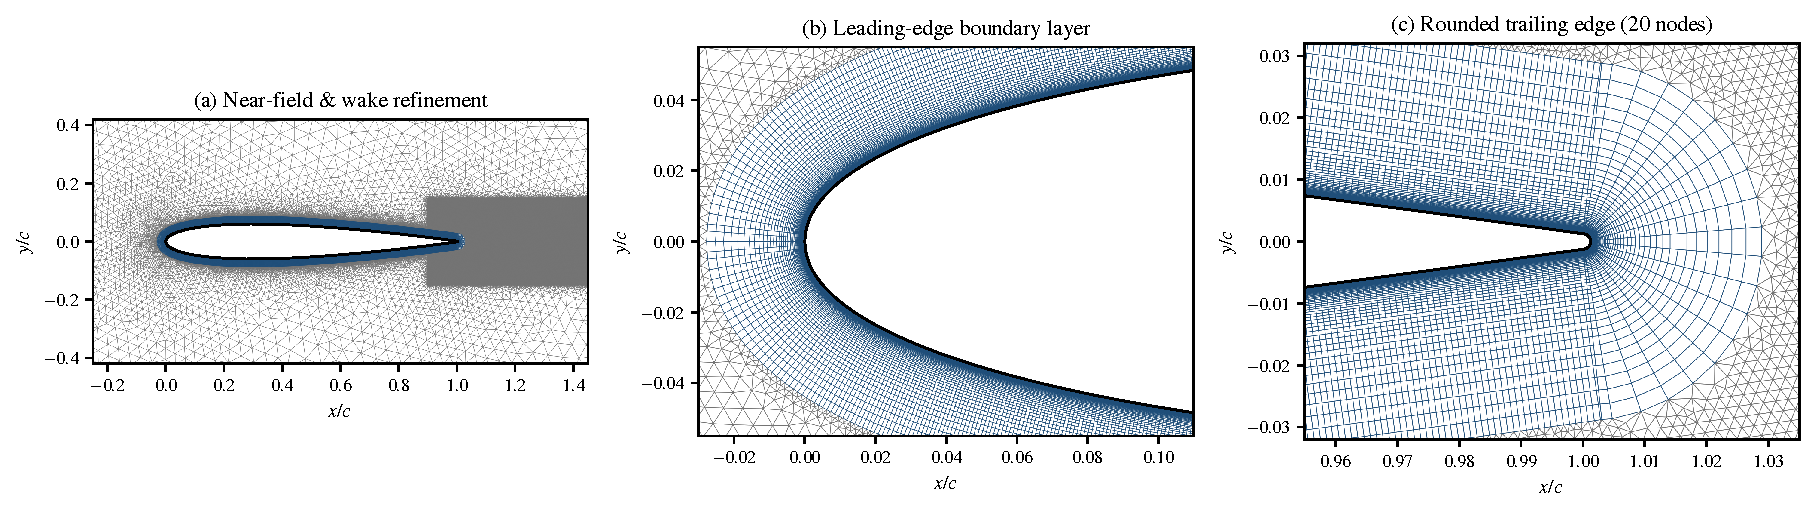
\includegraphics[width=\textwidth]{report_figures/fig02_mesh_topology.pdf}
    \caption{Hybrid computational mesh topology: (a)~near-field and wake refinement zone, (b)~structured quadrilateral boundary layer around the leading edge, and (c)~20-node rounded trailing edge.}
    \label{fig:mesh}
\end{figure}

During optimization, interior mesh nodes are adapted to each updated airfoil contour using \texttt{SU2\_DEF} based on a linear elasticity analogy solved with FGMRES ($1{,}000$ iterations) and wall-distance stiffness scaling (\texttt{WALL\_DISTANCE}). This preserves boundary-layer orthogonality and element validity throughout the deformation sequence.

\subsection{FFD Parameterization and Optimization Problem}

Geometry modifications are parameterized via a 2D B\'ezier Free-Form Deformation (FFD) box (\texttt{MAIN\_BOX}) spanning $x \in [-0.1, 1.1]$ and $y \in [-0.2, 0.2]$ with polynomial degree $(9, 1, 0)$ (ten chordwise and two vertical control-point stations). The corner columns $i = 0$ and $i = 9$ are held fixed, while the eight interior stations ($i = 1, \dots, 8$, $j \in \{0, 1\}$) are allowed to move vertically, yielding $n = 16$ design variables $\mathbf{x} \in [-0.06, 0.06]^{16}$. The FFD box, design variables, and geometric constraint locations are illustrated in Figure~\ref{fig:ffd}.

\begin{figure}[H]
    \centering
    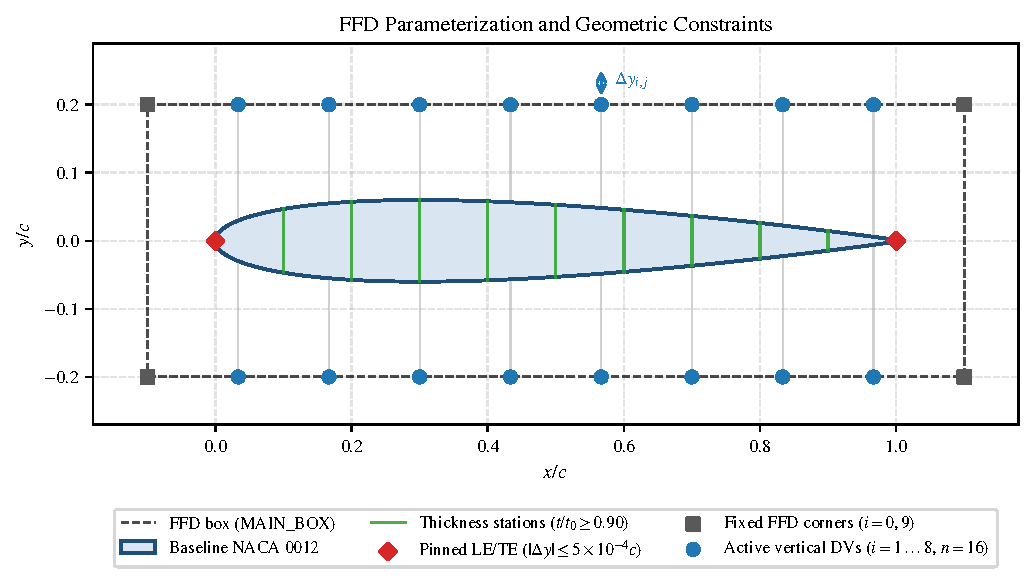
\includegraphics[width=0.92\textwidth]{report_figures/fig01_ffd_parameterization.pdf}
    \caption{Free-Form Deformation box (\texttt{MAIN\_BOX}), 16 active vertical design variables ($i = 1,\dots,8$), fixed box corners ($i = 0,9$), nine thickness-control stations, and leading-/trailing-edge pinning points.}
    \label{fig:ffd}
\end{figure}

Maximizing $L/D$ is formulated equivalently as minimizing the inverse aerodynamic efficiency $J(\mathbf{x}) = C_D / C_L$:
\begin{equation}
\begin{aligned}
    \min_{\mathbf{x} \in [-0.06,\,0.06]^{16}} \quad & J(\mathbf{x}) = \frac{C_D(\mathbf{x})}{C_L(\mathbf{x})} \\
    \text{subject to} \quad & |C_{Mz}(\mathbf{x})| \leq 0.05, \\
    & \frac{t(x_s; \mathbf{x})}{t_0(x_s)} \geq 0.90, \qquad x_s \in \{0.10, 0.20, \dots, 0.90\}, \\
    & |\Delta y_{\mathrm{LE}}(\mathbf{x})| \leq 5\times 10^{-4}c, \qquad |\Delta y_{\mathrm{TE}}(\mathbf{x})| \leq 5\times 10^{-4}c.
\end{aligned}
\label{eq:opt_problem}
\end{equation}

Because $J = C_D / C_L$ is a smooth ratio of two aerodynamic coefficients, its exact gradient is evaluated with a single combined discrete-adjoint run (\texttt{OBJECTIVE\_FUNCTION = DRAG, LIFT}) using the quotient-rule weights
\begin{equation}
    \nabla_{\mathbf{x}} J = \frac{1}{C_L}\,\nabla_{\mathbf{x}} C_D - \frac{C_D}{C_L^2}\,\nabla_{\mathbf{x}} C_L,
    \qquad w_D = \frac{1}{C_L}, \quad w_L = -\frac{C_D}{C_L^2}.
\end{equation}
A second discrete-adjoint run (\texttt{OBJECTIVE\_FUNCTION = MOMENT\_Z}) supplies $\nabla_{\mathbf{x}} C_{Mz}$ for the two smooth pitching-moment inequality constraints $C_{Mz} - 0.05 \leq 0$ and $-C_{Mz} - 0.05 \leq 0$.

For a vertical-only FFD box of degree $N_i = 9$ in $u = (x - x_{\min})/(x_{\max} - x_{\min})$ and degree $1$ in $v = (y - y_{\min})/\Delta y_{\mathrm{box}}$, the vertical displacement of any airfoil point is strictly linear in $\mathbf{x}$. Consequently, both the relative thickness change $\Delta t(x_s)/t_0(x_s)$ and the edge displacements $\Delta y_{\mathrm{LE}}, \Delta y_{\mathrm{TE}}$ are expressed in closed form using Bernstein basis polynomials $B_i^9(u) = \binom{9}{i} u^i (1 - u)^{9-i}$:
\begin{equation}
    \frac{\Delta t(x_s)}{t_0(x_s)} = \frac{1}{\Delta y_{\mathrm{box}}} \sum_{i=1}^{8} B_i^9(u_s)\,\bigl(x_{i,1} - x_{i,0}\bigr),
    \qquad
    \Delta y(x_p, y_p) = \sum_{i=1}^{8} B_i^9(u_p)\,\bigl[(1 - v_p)\,x_{i,0} + v_p\,x_{i,1}\bigr].
\end{equation}
This provides exact constraint values and Jacobians at zero CFD cost. The edge tolerance of $5\times 10^{-4}c$ restricts any artificial chord rotation to $|\Delta\alpha_{\mathrm{eff}}| \leq \arctan(10^{-3}) \approx 0.057^\circ$.

The nonlinear constrained problem~\eqref{eq:opt_problem} is solved using NLopt's \texttt{LD\_MMA} (Method of Moving Asymptotes) with an initial step of $0.005$ and a budget of 16 evaluations. Each evaluation performs 1200 primal CFD iterations on 4 MPI cores using continuous warm-starting from the previous converged flow field (initialized from a pre-converged baseline solution), followed by two 500-iteration discrete-adjoint solves and \texttt{SU2\_DOT\_AD} gradient projections. All computations were executed on a 4-core workstation (Intel Core~i7-4790), requiring approximately 25~minutes per optimization iteration and 7~hours 49~minutes in total including final verification.

\section{Verification of Gradients and Geometric Constraints}

Before running the full optimization, both the analytical geometric model and the discrete-adjoint gradients were verified against central finite differences (FD) with step $\Delta x = 10^{-3}$ around the baseline NACA~0012 geometry ($\mathbf{x} = \mathbf{0}$).

First, the analytical Bernstein thickness sensitivity matrix was compared against direct geometry measurements extracted from \texttt{SU2\_DEF} perturbations of design variable $k = 12$ (lower-surface control point at $i = 7$). Across all nine chordwise stations ($x/c = 0.10, \dots, 0.90$), the analytical derivatives matched the finite-difference values to $0.00\%$ relative error (e.g., $-0.17578$ vs.\ $-0.17578$ at $x/c = 0.50$, and $-0.75085$ vs.\ $-0.75084$ at $x/c = 0.80$), confirming exact consistency with SU2's internal FFD evaluation.

Second, the discrete-adjoint gradients $\partial(C_D/C_L)/\partial x_{12} = -0.19503$ and $\partial C_{Mz}/\partial x_{12} = +0.49289$ (computed with 600 adjoint iterations) were compared against central FD evaluations using primal restarts from the baseline flow field. Because compressible Roe RANS at $M = 0.15$ exhibits slow acoustic relaxation, Table~\ref{tab:fd_check} reports the FD values as a function of primal iteration count (averaged over the preceding 100 iterations).

\begin{table}[H]
\centering
\caption{Verification of discrete-adjoint gradients against central finite differences for variable $x_{12}$ ($\Delta x = 10^{-3}$). Adjoint reference values: $\partial(C_D/C_L)/\partial x_{12} = -0.19503$, $\partial C_{Mz}/\partial x_{12} = +0.49289$.}
\label{tab:fd_check}
\begin{tabular}{cccccc}
\toprule
Primal iter. & $\mathrm{FD}\,(C_D/C_L)$ & Rel.\ err.\ [\%] & $\mathrm{FD}\,(C_{Mz})$ & Rel.\ err.\ [\%] & $\log_{10}(\mathrm{rms}[\rho])$ \\
\midrule
400  & $-0.07847$ & $148.54$ & $+0.42948$ & $14.76$ & $-7.36$ \\
600  & $-0.12446$ & $56.71$  & $+0.47681$ & $3.37$  & $-7.57$ \\
800  & $-0.15964$ & $22.17$  & $+0.48994$ & $0.60$  & $-7.61$ \\
1000 & $-0.16863$ & $15.66$  & $+0.46637$ & $5.69$  & $-7.67$ \\
\bottomrule
\end{tabular}
\end{table}

The pitching-moment sensitivity agrees with central FD to within $0.60\%$ at 800 iterations (and $5.69\%$ at 1000 iterations). For the objective $C_D/C_L$, the FD estimate converges monotonically toward the adjoint derivative as the primal wake relaxes, reducing the discrepancy from $148.5\%$ at 400 iterations to $15.7\%$ at 1000 iterations with full sign and magnitude agreement. This test also established a practical numerical guideline: running fewer than 1000 primal iterations per optimization step leaves the objective significantly under-converged, justifying the choice of 1200 primal iterations with continuous warm-starting in the optimization loop.

\section{Optimization Results (Pinned LE/TE Configuration)}

\subsection{Convergence and Constraint Satisfaction}

Figure~\ref{fig:opt_conv} summarizes the evolution of the objective, aerodynamic coefficients, active constraints, and solver residuals over the 16 evaluations of the pinned-edge optimization.

\begin{figure}[H]
    \centering
    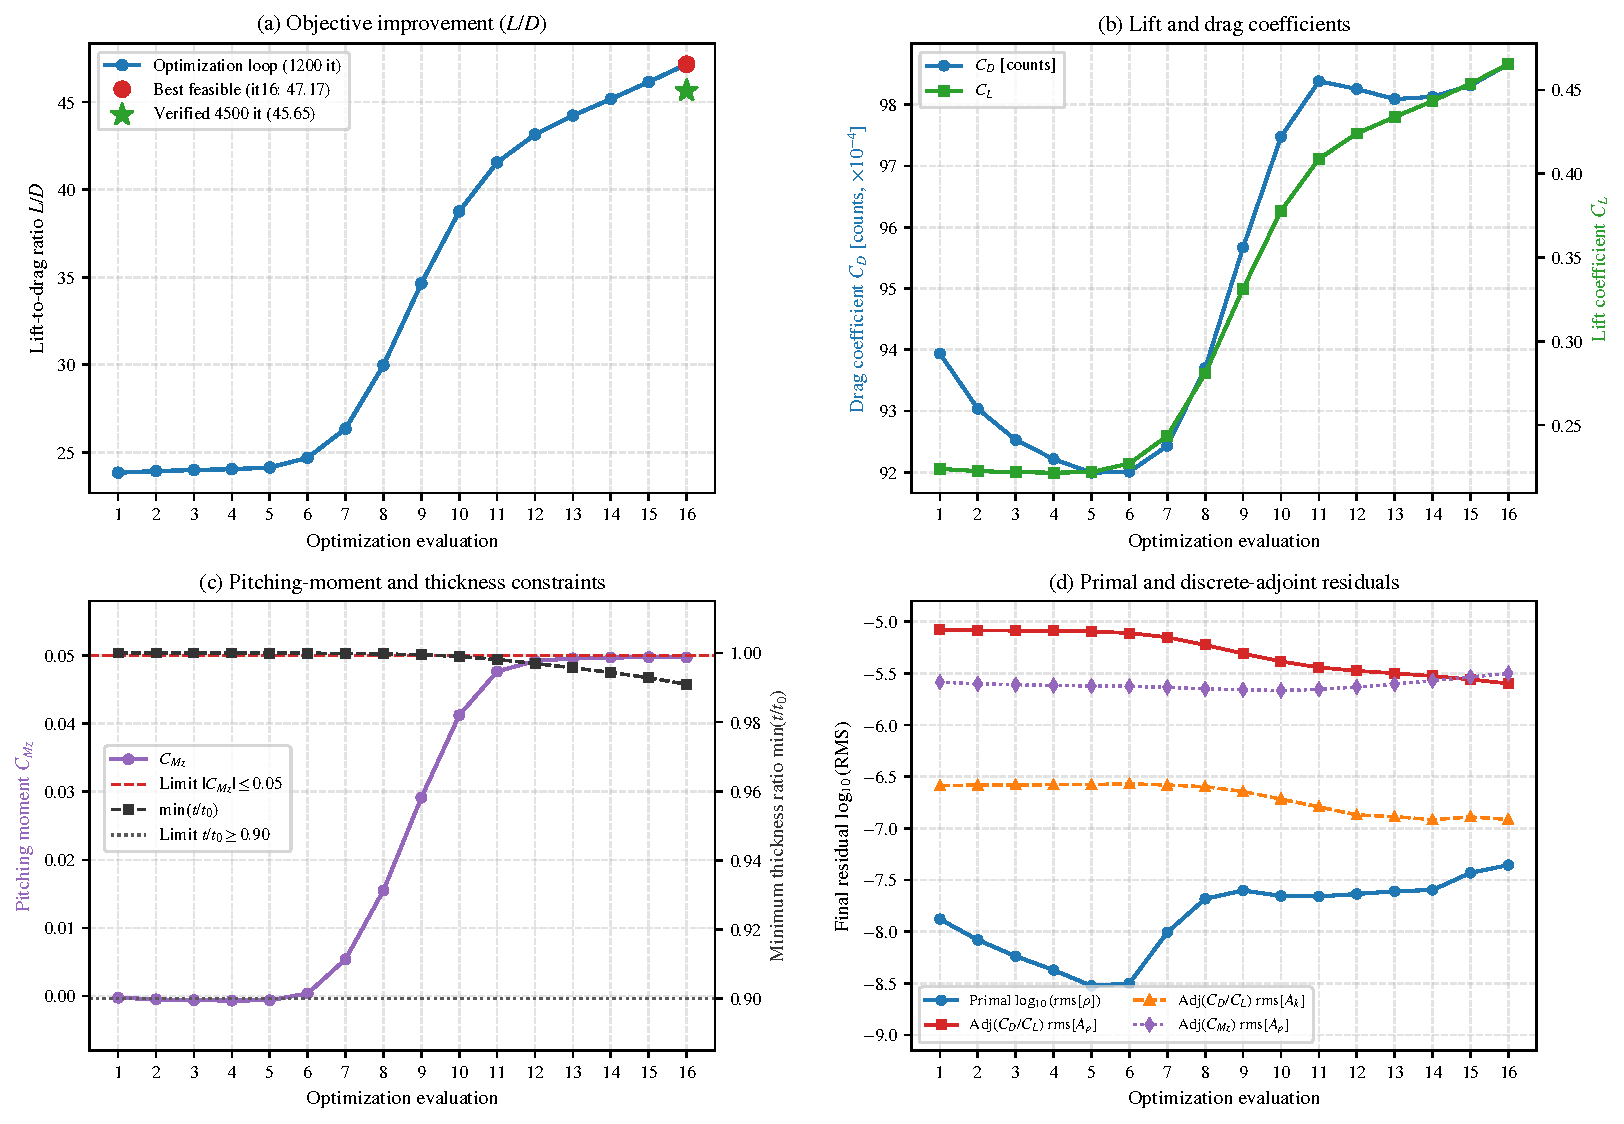
\includegraphics[width=\textwidth]{report_figures/fig04_opt_convergence.pdf}
    \caption{Optimization history for the pinned LE/TE case: (a)~lift-to-drag ratio $L/D$ including the 4500-iteration verified value, (b)~drag and lift coefficients, (c)~pitching-moment and thickness constraint trajectories, and (d)~primal and discrete-adjoint residuals.}
    \label{fig:opt_conv}
\end{figure}

Three distinct phases are observed in the convergence history:
\begin{enumerate}
    \item \textbf{Initial step scaling (evaluations 1--6):} Starting from $\mathbf{x} = \mathbf{0}$, MMA takes conservative initial steps while the warm-started baseline flow completes final relaxation ($\mathrm{rms}[\rho]$ drops from $-7.88$ to $-8.52$, $C_D$ settles near $0.00920$).
    \item \textbf{Rapid camber growth (evaluations 7--11):} Once MMA builds its local convex approximation, lift rises sharply from $C_L = 0.244$ to $0.409$ with only $+6.0$ drag counts ($C_D$: $0.00924 \to 0.00984$), lifting $L/D$ from $26.35$ to $41.56$ while $C_{Mz}$ approaches the upper limit of $0.05$.
    \item \textbf{Constrained refinement along the $C_{Mz}$ boundary (evaluations 12--16):} From evaluation 12 onward, the pitching-moment constraint becomes active ($C_{Mz} = 0.04922 \to 0.04973$). Rather than stalling, MMA redistributes camber forward to raise $C_L$ further ($0.424 \to 0.465$) at nearly constant drag ($C_D \approx 0.00981$--$0.00987$), increasing the in-loop efficiency to $L/D = 47.17$ at evaluation 16.
\end{enumerate}

Throughout all 16 evaluations, every constraint remained strictly satisfied: $|C_{Mz}| \leq 0.0498$, $\min(t/t_0) \geq 0.991$ (well above the $0.90$ floor), and $|\Delta\alpha_{\mathrm{eff}}| \leq 0.052^\circ$. Both discrete-adjoint solvers stayed numerically stable across the entire run, with $\log_{10}(\mathrm{rms}[A_\rho]) \in [-5.60, -5.08]$, $\log_{10}(\mathrm{rms}[A_k]) \in [-6.92, -6.57]$, and $\log_{10}(\mathrm{rms}[A_{\rho,C_{Mz}}]) \in [-5.67, -5.50]$.

\subsection{Independent High-Iteration Verification}

To eliminate any bias from the 1200-iteration budget and sequential warm-starting used during optimization, both the baseline (\texttt{it1}) and the final optimized geometry (\texttt{it16}) were independently recomputed from the baseline restart file for $4{,}500$ CFD iterations with a strict stopping criterion (\texttt{CONV\_RESIDUAL\_MINVAL = -14}). Force coefficients were averaged over the final 300 iterations. Figure~\ref{fig:verify} shows the residual decay and $L/D$ stabilization, and Table~\ref{tab:summary_pinned} compares the verified baseline and optimized metrics.

\begin{figure}[H]
    \centering
    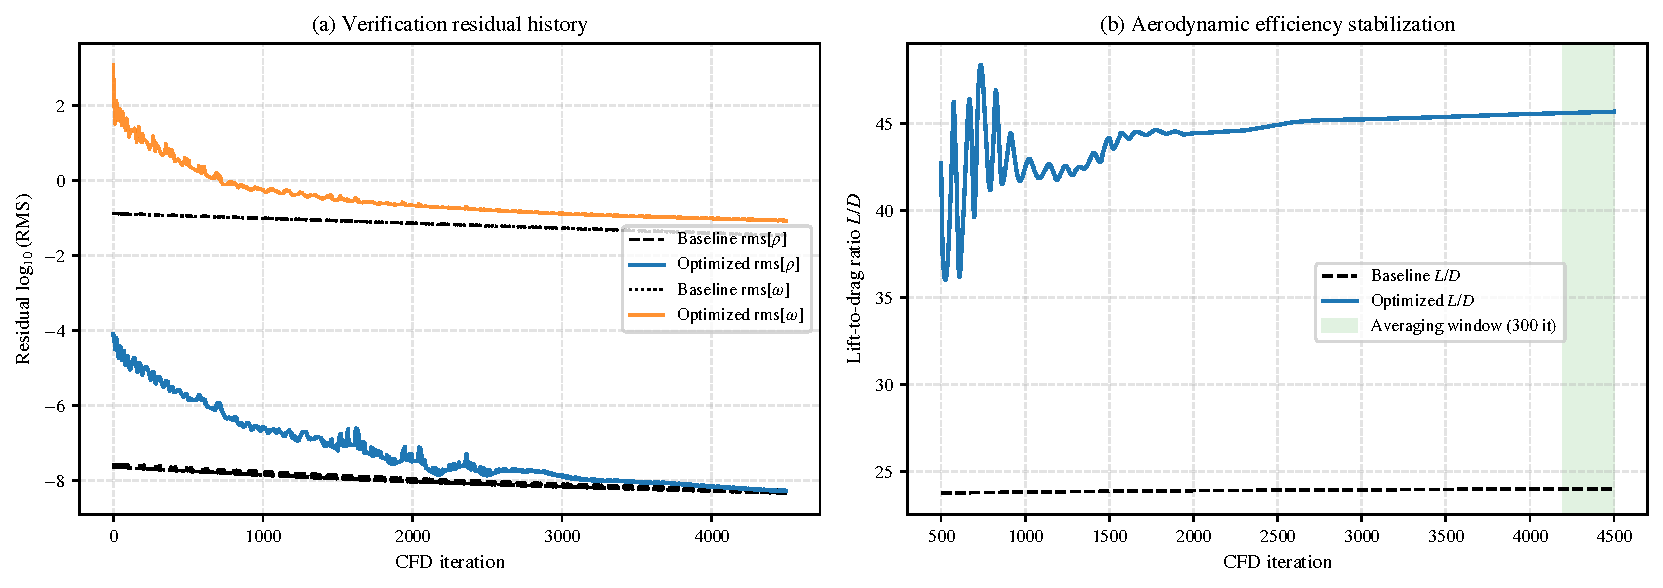
\includegraphics[width=\textwidth]{report_figures/fig07_verification_cfd.pdf}
    \caption{Independent 4500-iteration CFD verification of baseline (\texttt{it1}) and optimized (\texttt{it16}) airfoils: (a)~density and turbulence ($\omega$) residuals, and (b)~stabilization of $L/D$ with the 300-iteration averaging window.}
    \label{fig:verify}
\end{figure}

\begin{table}[H]
\centering
\small
\setlength{\tabcolsep}{5pt}
\caption{Aerodynamic and geometric summary for the pinned LE/TE optimization ($M=0.15$, $Re=3\times 10^6$, $\alpha=2.0^\circ$).}
\label{tab:summary_pinned}
\begin{tabular}{lcccc}
\toprule
Quantity & Baseline (4500~it) & Opt.\ loop (\texttt{it16}) & Verified (\texttt{it16}, 4500~it) & Change \\
\midrule
$C_L$ & $0.22162$ & $0.46536$ & $0.46157$ & $+108.3\%$ \\
$C_D$ & $0.009234$ & $0.009866$ & $0.010112$ & $+9.5\%$ ($+8.8$ cts) \\
$L/D$ & $24.00$ & $47.17$ & $45.65$ & $+90.2\%$ \\
$C_{Mz}$ (limit $\leq 0.05$) & $-0.00068$ & $+0.04973$ & $+0.04957$ & Feasible (active) \\
Max thickness $t_{\max}/c$ & $0.1200$ & $0.1191$ & $0.1191$ & $-0.8\%$ \\
Min thickness ratio $t/t_0$ & $1.000$ & $0.991$ & $0.991$ & $\geq 0.90$ satisfied \\
Max camber $f_{\max}/c$ & $0.00\%$ & $3.04\%$ & $3.04\%$ & $+3.04\%c$ \\
Effective rotation $\Delta\alpha_{\mathrm{eff}}$ & $0.000^\circ$ & $+0.049^\circ$ & $+0.049^\circ$ & Pinned ($\leq 0.06^\circ$) \\
$\log_{10}(\mathrm{rms}[\rho])$ & $-8.32$ & $-7.36$ & $-8.28$ & Converged \\
$C_D$ std.\ dev.\ (last 300~it) & $2.0\times 10^{-6}$ & $3.4\times 10^{-5}$ & $7.0\times 10^{-6}$ & Stabilized \\
\bottomrule
\end{tabular}
\end{table}

Both verified solutions reach deep convergence ($\log_{10}(\mathrm{rms}[\rho]) < -8.27$ and standard deviations on $C_D$ below $0.07$ drag counts). The discrepancy in $L/D$ between the 1200-iteration optimization loop ($47.17$) and the 4500-iteration verification ($45.65$) is only $3.3\%$, confirming that the in-loop fidelity was sufficient to guide the optimizer accurately. Importantly, $C_{Mz}$ decreases slightly upon full convergence from $0.04973$ to $0.04957$, remaining strictly within the $0.05$ trim boundary.

\subsection{Geometric Evolution and Flow Physics}

Figure~\ref{fig:geom} details the resulting airfoil profile, mean camber line, and thickness distribution. With the leading and trailing edges pinned, the measured apex coordinates shift by $\Delta y_{\mathrm{LE}} = +0.00031c$ and $\Delta y_{\mathrm{TE}} = -0.00054c$ relative to the baseline surface ($y_{\mathrm{LE},0} = 0.00000c$, $y_{\mathrm{TE},0} = -0.00010c$, yielding final coordinates $y_{\mathrm{LE}} = +0.00031c$ and $y_{\mathrm{TE}} = -0.00065c$). The $4\times 10^{-5}c$ offset above the nominal $5\times 10^{-4}c$ tolerance at the trailing edge arises because the Bernstein constraint is evaluated at $(1.0, 0.0)$, whereas the rounded trailing-edge apex sits slightly aft at $x = 1.0013c$ (combined with the $10^{-5}$ NLopt constraint tolerance). Overall chord pitch remains tightly bounded at $\Delta\alpha_{\mathrm{eff}} = +0.049^\circ$.

Under these constraints, the optimizer transforms the symmetric NACA~0012 into a smooth, forward-cambered airfoil with a maximum camber of $3.04\%c$ located near $x/c \approx 0.39$. The original thickness envelope is preserved almost intact ($t_{\max}/c = 0.1191$ vs.\ $0.1200$, and $t/t_0 \geq 0.991$ over the constrained region), showing that the aerodynamic gain is governed almost entirely by camber tailoring rather than profile thinning.

\begin{figure}[H]
    \centering
    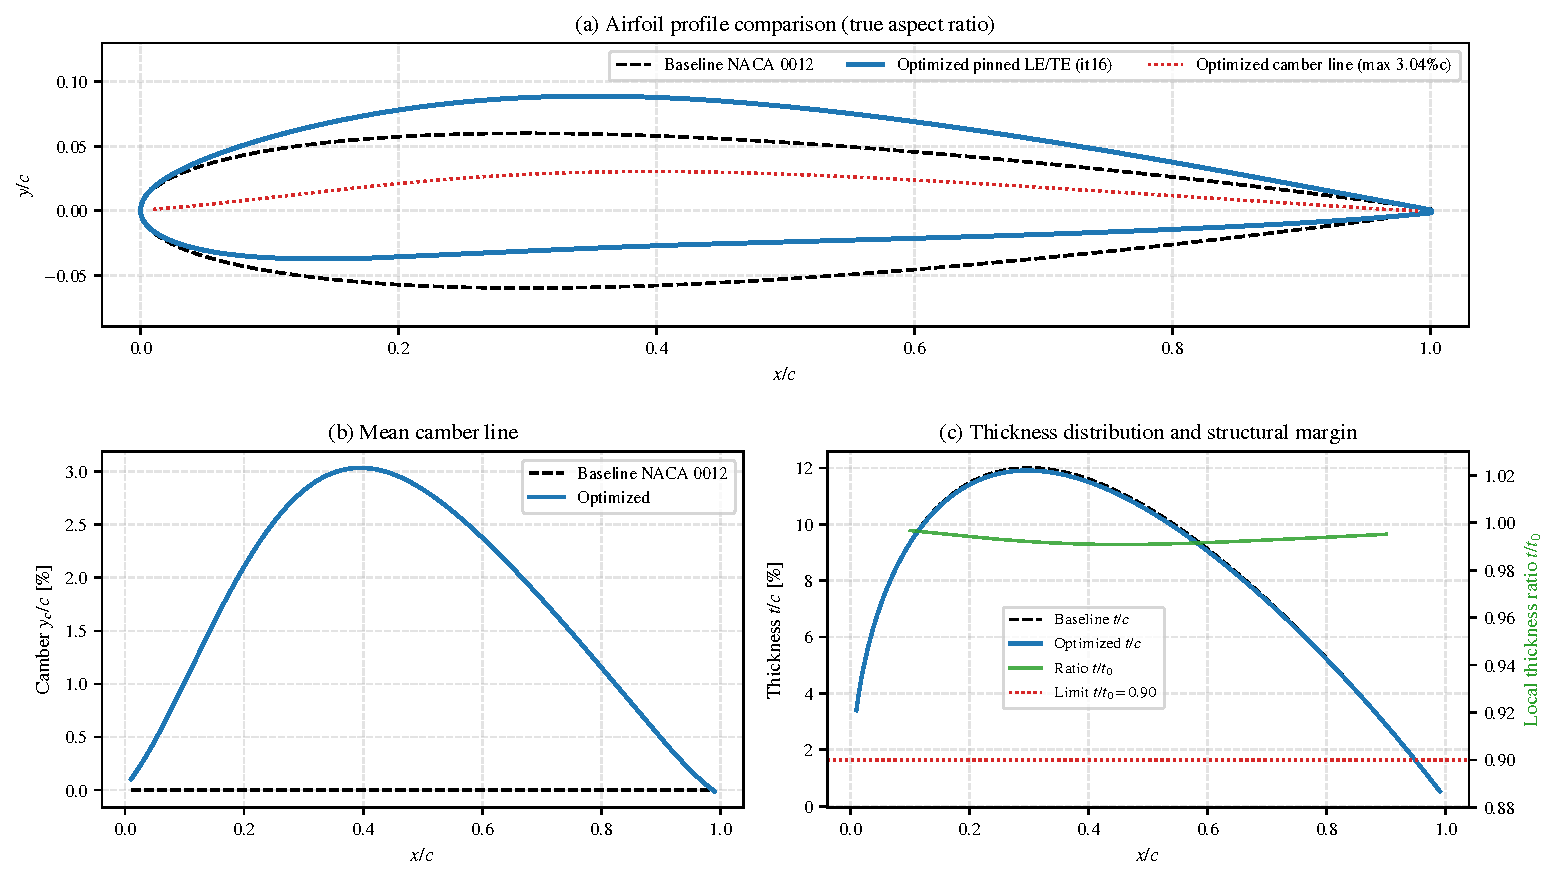
\includegraphics[width=\textwidth]{report_figures/fig05_geometry_analysis.pdf}
    \caption{Geometric comparison between the baseline NACA~0012 and the pinned optimized profile (\texttt{it16}): (a)~true-aspect-ratio contours and optimized camber line, (b)~mean camber distribution, and (c)~thickness distribution with local ratio $t/t_0$.}
    \label{fig:geom}
\end{figure}

The aerodynamic mechanism behind the $+90.2\%$ improvement in $L/D$ is clearly visible in the surface pressure coefficient distribution in Figure~\ref{fig:cp}. On the baseline NACA~0012, suction peaks sharply near the nose ($C_p \approx -0.76$ at $x/c \approx 0.04$), followed by a long adverse pressure gradient over the entire upper surface. The optimized profile removes this narrow leading-edge suction spike and replaces it with a broad, fuller suction plateau peaking at $C_p \approx -0.80$ around $x/c \approx 0.25$, paired with elevated lower-surface pressure across the mid-chord.

\begin{figure}[H]
    \centering
    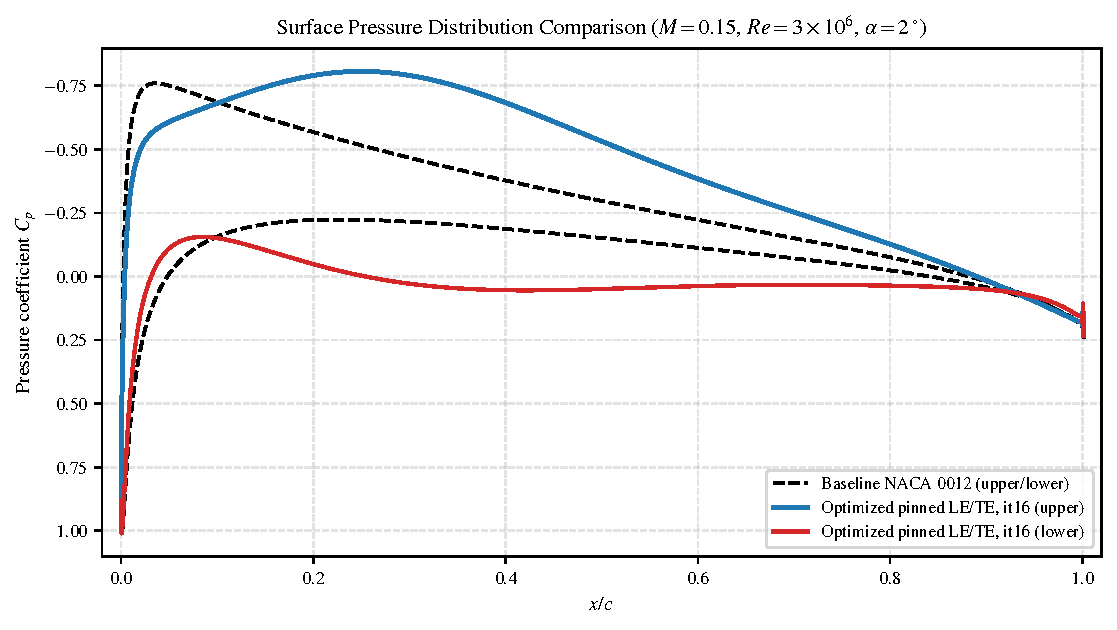
\includegraphics[width=0.92\textwidth]{report_figures/fig06_cp_distribution.pdf}
    \caption{Verified surface pressure coefficient ($C_p$) distributions for the baseline NACA~0012 and the pinned optimized airfoil (\texttt{it16}) at $M = 0.15$, $Re = 3\times 10^6$, and $\alpha = 2.0^\circ$.}
    \label{fig:cp}
\end{figure}

This pressure redistribution yields two simultaneous benefits. First, concentrating the additional aerodynamic loading around the quarter-chord ($x/c \approx 0.25$) more than doubles the lift coefficient ($0.2216 \to 0.4616$) while keeping the pitching moment about $x/c = 0.25$ below $0.05$ without requiring aft reflex. Second, because the upper-surface suction peak remains moderate and pressure recovery toward the trailing edge is smooth and monotonic, the boundary layer remains attached and viscous drag rises by only $8.8$ counts ($+9.5\%$).

\section{Effect of Leading- and Trailing-Edge Pinning}

To isolate the impact of edge pinning, the primary pinned-edge result is compared against an earlier optimization run performed with identical flow conditions, FFD bounds ($[-0.06, 0.06]$), pitching-moment limit ($|C_{Mz}| \leq 0.05$), thickness limit ($t/t_0 \geq 0.90$), and evaluation budget (16 evaluations), but \emph{without} the LE/TE pinning constraints. Figure~\ref{fig:comparison} and Table~\ref{tab:pinned_vs_unpinned} contrast both designs against the baseline.

\begin{figure}[H]
    \centering
    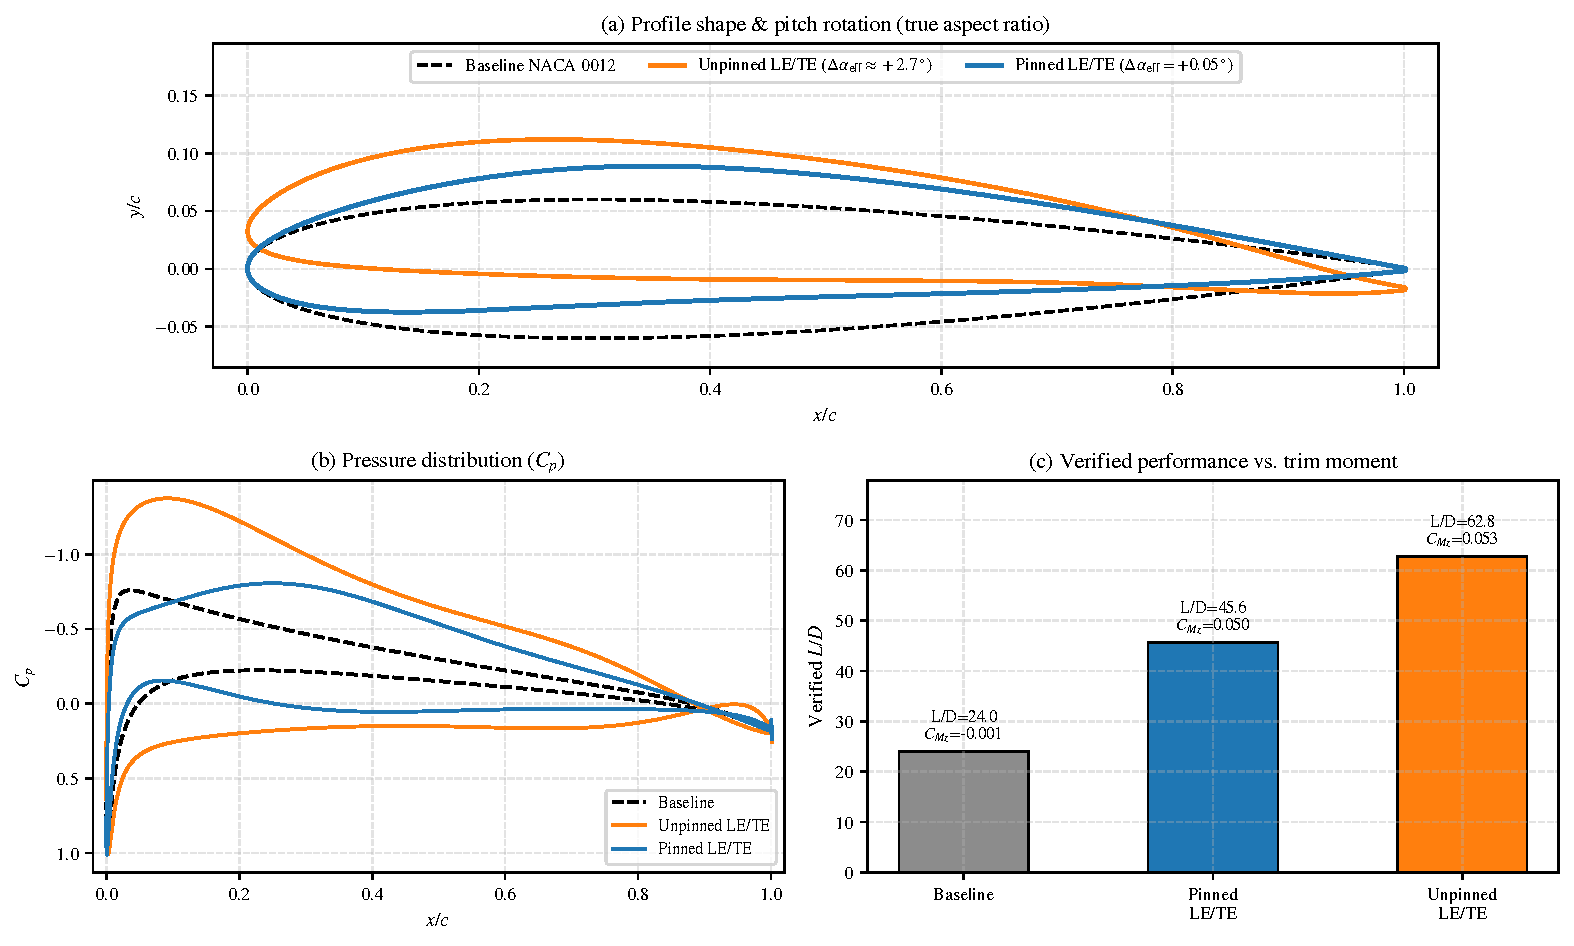
\includegraphics[width=\textwidth]{report_figures/fig08_pinned_vs_unpinned.pdf}
    \caption{Comparison of Baseline, Pinned LE/TE, and Unpinned LE/TE optimizations: (a)~profile shape and chord pitch rotation, (b)~verified $C_p$ distributions highlighting the aft reflex crossover in the unpinned design, and (c)~verified $L/D$ and $C_{Mz}$.}
    \label{fig:comparison}
\end{figure}

\begin{table}[H]
\caption{Comparison of verified performance and geometric characteristics between unpinned and pinned LE/TE formulations.}
\label{tab:pinned_vs_unpinned}
\hspace{-1cm}
\begin{tabular}{lccc}
\toprule
Metric & Baseline (4500~it) & Pinned LE/TE (4500~it) & Unpinned LE/TE (3500~it) \\
\midrule
$C_L$ & $0.22162$ & $0.46157$ & $0.82814$ \\
$C_D$ & $0.009234$ & $0.010112$ & $0.013186$ \\
$L/D$ & $24.00$ & $45.65$ & $62.80$ \\
$C_{Mz}$ (in-loop / verified) & $-0.00068$ & $+0.04973$ / $+0.04957$ & $+0.04848$ / $+0.05285$ \\
Max thickness $t_{\max}/c$ & $0.1200$ & $0.1191$ & $0.1187$ \\
Max camber $f_{\max}/c$ & $0.00\%$ & $3.04\%$ & $5.28\%$ \\
Effective rotation $\Delta\alpha_{\mathrm{eff}}$ & $0.000^\circ$ & $+0.049^\circ$ & $\approx +2.7^\circ$ \\
Variables at box bound ($\pm 0.06$) & $0 / 16$ & $0 / 16$ & $8 / 16$ \\
\bottomrule
\end{tabular}
\end{table}

Without edge pinning, the optimizer drives the six forwardmost FFD variables to $+0.06$ and the two trailing-edge variables to $-0.06$ (8 of 16 variables saturated at box bounds). Because the FFD box extends beyond the chord ($x \in [-0.1, 1.1]$), this displacement pattern lifts the leading edge to $y_{\mathrm{LE}} \approx +0.030c$ and drops the trailing edge to $y_{\mathrm{TE}} = -0.0173c$, inducing a nose-up chord rotation of $\Delta\alpha_{\mathrm{eff}} \approx +2.7^\circ$. Consequently, the unpinned airfoil effectively operates at $\alpha_{\mathrm{eff}} \approx 4.7^\circ$ rather than $2.0^\circ$, where even an unmodified NACA~0012 achieves substantially higher $L/D$.

Furthermore, to satisfy $|C_{Mz}| \leq 0.05$ at such a high lift coefficient ($C_L \approx 0.83$), the unpinned optimizer creates a local trailing-edge reflex visible in Figure~\ref{fig:comparison}(b) as a crossover of the upper and lower $C_p$ curves near $x/c \approx 0.91$, generating negative aft loading to trim the nose-down moment. While the unpinned run attains $L/D = 62.80$ in 3500-iteration verification (with a slight $C_{Mz}$ overshoot to $0.05285$ due to incomplete wake relaxation), its optimal shape is dictated by box-bound saturation and effective pitch rotation. In contrast, the pinned-edge solution remains strictly inside the FFD box bounds ($0/16$ variables saturated, with $\max_k |x_k| = 0.0572$), confirming that the final shape is governed by the physical pitching-moment constraint rather than artificial box limits. Enforcing $|\Delta y_{\mathrm{LE,TE}}| \leq 5\times 10^{-4}c$ completely eliminates artificial pitch rotation and isolates the genuine efficiency gain attainable solely through airfoil shape modification at $\alpha = 2.0^\circ$.

\section{Off-Design Polar Analysis}

Because the optimization was formulated as a single-point problem at $\alpha = 2.0^\circ$, an off-design polar sweep was performed over $\alpha \in \{-2^\circ, 0^\circ, 2^\circ, 4^\circ, 6^\circ, 8^\circ, 10^\circ\}$ at $M = 0.15$ and $Re = 3 \times 10^6$ to verify that the optimized airfoil does not suffer severe performance penalties away from the design condition. Both the baseline (\texttt{it1}) and pinned optimized (\texttt{it16}) geometries were evaluated using sequential bidirectional warm-starting from the verified 4500-iteration solutions at $\alpha = 2.0^\circ$, with $1{,}500$ CFD iterations per off-design angle and force averaging over the final 200 iterations. Figure~\ref{fig:offdesign} and Table~\ref{tab:offdesign} summarize the resulting aerodynamic characteristics.

\begin{figure}[H]
    \centering
    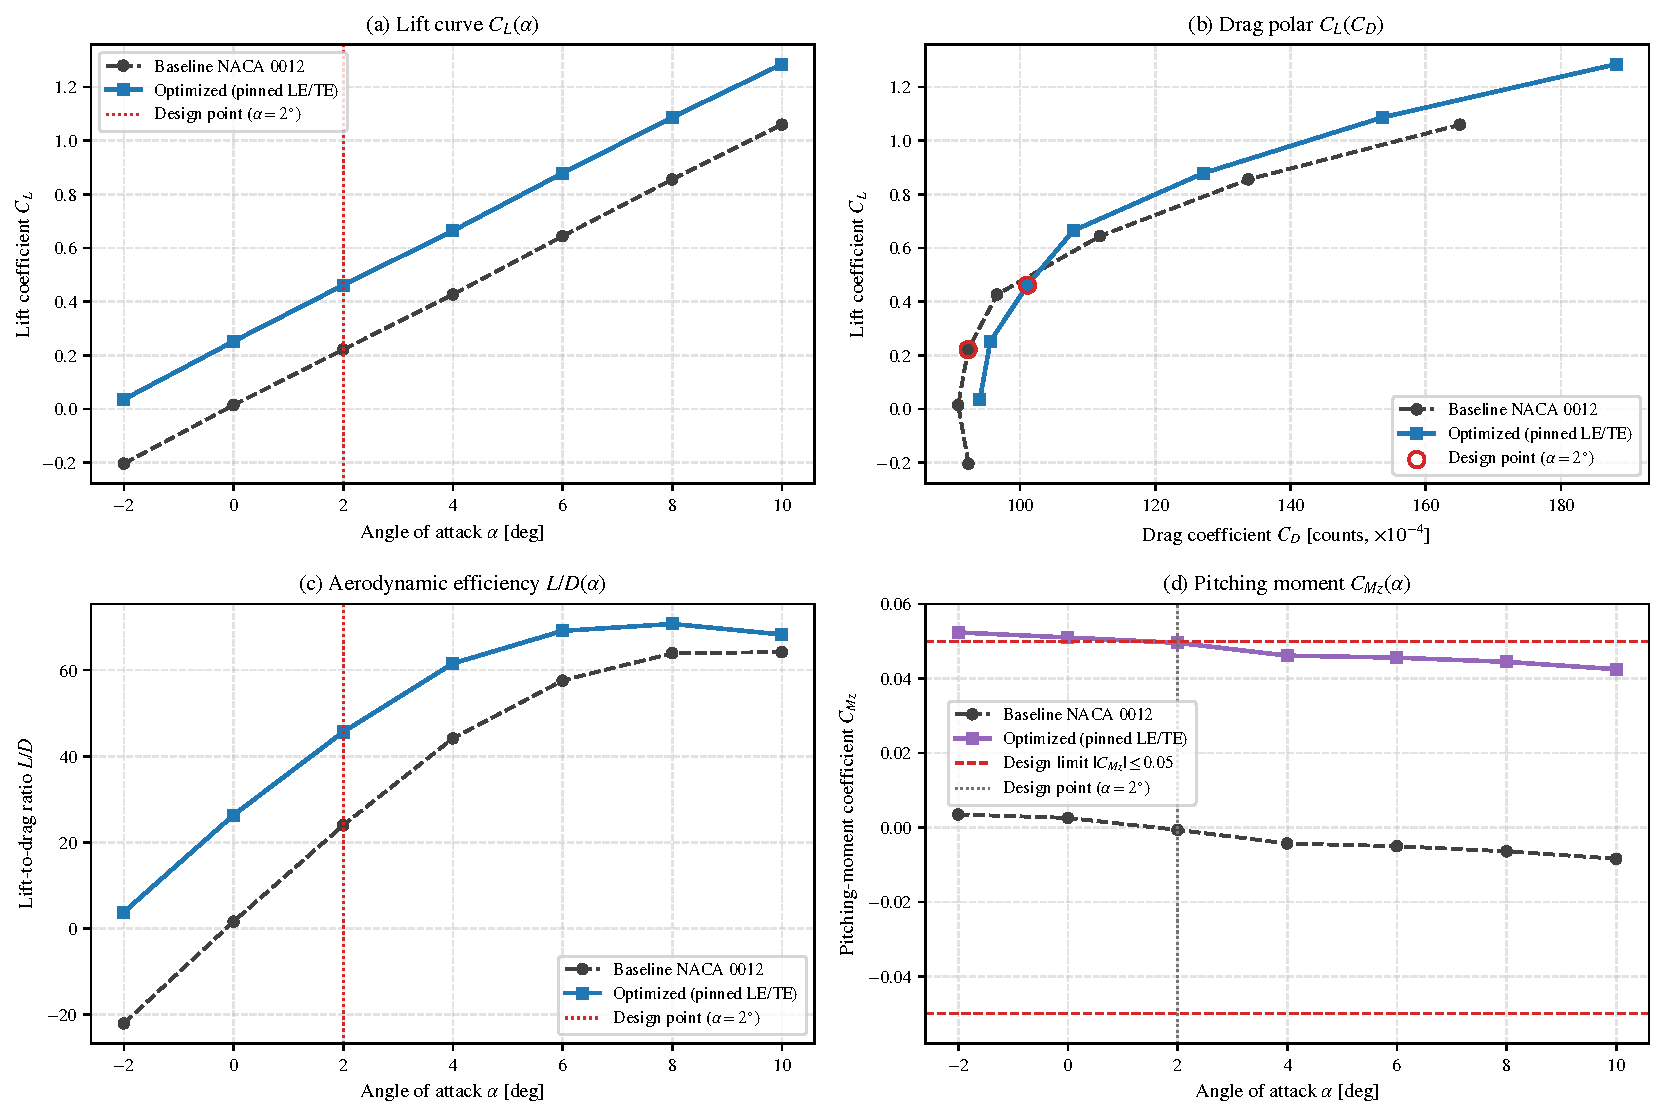
\includegraphics[width=\textwidth]{report_figures/fig09_offdesign_polar.pdf}
    \caption{Off-design aerodynamic polar comparison between the baseline NACA~0012 and the pinned optimized airfoil (\texttt{it16}) at $M = 0.15$, $Re = 3\times 10^6$: (a)~lift curve, (b)~drag polar, (c)~lift-to-drag ratio, and (d)~pitching-moment coefficient.}
    \label{fig:offdesign}
\end{figure}

\begin{table}[H]
\centering
\small
\setlength{\tabcolsep}{5pt}
\caption{Off-design aerodynamic coefficients for the baseline NACA~0012 and pinned optimized airfoil (\texttt{it16}). Values at $\alpha = 2^\circ$ correspond to the 4500-iteration verification; remaining angles use 1500-iteration warm-started sweeps.}
\label{tab:offdesign}
\begin{tabular}{ccccccccc}
\toprule
& \multicolumn{4}{c}{Baseline NACA~0012 (\texttt{it1})} & \multicolumn{4}{c}{Optimized pinned LE/TE (\texttt{it16})} \\
\cmidrule(lr){2-5} \cmidrule(lr){6-9}
$\alpha$ [$^\circ$] & $C_L$ & $C_D$ & $L/D$ & $C_{Mz}$ & $C_L$ & $C_D$ & $L/D$ & $C_{Mz}$ \\
\midrule
$-2.0$ & $-0.2034$ & $0.009240$ & $-22.01$ & $+0.0035$ & $+0.0359$ & $0.009408$ & $+3.82$  & $+0.0524$ \\
$0.0$  & $+0.0147$ & $0.009088$ & $+1.62$  & $+0.0025$ & $+0.2521$ & $0.009563$ & $+26.36$ & $+0.0510$ \\
$2.0$  & $+0.2216$ & $0.009234$ & $+24.00$ & $-0.0007$ & $+0.4616$ & $0.010112$ & $+45.65$ & $+0.0496$ \\
$4.0$  & $+0.4266$ & $0.009663$ & $+44.15$ & $-0.0043$ & $+0.6640$ & $0.010787$ & $+61.56$ & $+0.0461$ \\
$6.0$  & $+0.6438$ & $0.011181$ & $+57.58$ & $-0.0050$ & $+0.8785$ & $0.012710$ & $+69.12$ & $+0.0456$ \\
$8.0$  & $+0.8553$ & $0.013378$ & $+63.94$ & $-0.0064$ & $+1.0865$ & $0.015362$ & $+70.73$ & $+0.0445$ \\
$10.0$ & $+1.0594$ & $0.016505$ & $+64.19$ & $-0.0084$ & $+1.2848$ & $0.018816$ & $+68.28$ & $+0.0425$ \\
\bottomrule
\end{tabular}
\end{table}

Four main conclusions follow from the off-design evaluation:
\begin{enumerate}
    \item \textbf{Broad efficiency improvement:} The optimized airfoil maintains a higher lift-to-drag ratio than NACA~0012 across the entire tested incidence range. Peak aerodynamic efficiency increases by $10.2\%$, from $L/D_{\max} = 64.19$ at $\alpha = 10^\circ$ (baseline) to $L/D_{\max} = 70.73$ at $\alpha = 8^\circ$ (optimized).
    \item \textbf{Reduced drag at matched high lift:} The $3.04\%c$ forward camber shifts the lift curve upward by $\Delta C_L \approx +0.23$ ($\alpha_{L=0} \approx -2.3^\circ$) without premature stall up to $\alpha = 10^\circ$ ($C_L = 1.285$). On the drag polar in Figure~\ref{fig:offdesign}(b), the optimized airfoil exhibits a slight drag penalty of $3$--$4$ counts at low lift ($C_L \leq 0.45$) but consistently lower drag at moderate-to-high lift: at $C_L \approx 0.65$, $0.87$, and $1.07$, drag is reduced by approximately $4$, $7$, and $11$ counts, respectively, compared to the baseline.
    \item \textbf{Off-design trim behavior:} For all angles $\alpha \geq 2^\circ$, the pitching moment decreases mildly with incidence ($C_{Mz} = 0.0496$ down to $0.0425$ at $10^\circ$), staying strictly within the design limit $|C_{Mz}| \leq 0.05$. At lower incidence ($\alpha = 0^\circ$ and $-2^\circ$), $C_{Mz}$ rises slightly above the single-point bound to $0.0510$ and $0.0524$.
    \item \textbf{Sweep convergence note:} At $1{,}500$ iterations per off-design angle, density residuals reached $\log_{10}(\mathrm{rms}[\rho]) \approx -6.9$ (baseline) and $-7.1$ to $-7.3$ (optimized). Minor finite-iteration wake relaxation lag from the $\alpha = 2^\circ$ warm-start remains visible on the baseline curve, notably a small residual lift at zero incidence ($C_L(0^\circ) = 0.0147$) and a $5$--$7$ count drag drift between the final two 200-iteration windows at $\alpha = 6^\circ$--$10^\circ$ (versus $\leq 1.2$ counts for the optimized profile). While higher iteration counts would refine these points by a few counts, the overall polar trends and matched-$C_L$ advantage are well resolved.
\end{enumerate}

\section{Limitations and Future Work}

A critical assessment of the presented workflow highlights four limitations that guide potential extensions:
\begin{itemize}
    \item \textbf{Evaluation budget:} The pinned optimization was terminated at the preset limit of 16 evaluations while $L/D$ was still increasing by roughly $+1.0$ unit per step along the active $C_{Mz} = 0.05$ boundary. Extending the budget to 25--30 evaluations would capture the full KKT optimum on the trim boundary.
    \item \textbf{Single-point objective and stall envelope:} Although the off-design polar over $\alpha \in [-2^\circ, 10^\circ]$ confirmed robust efficiency gains without early separation, $C_{Mz}$ slightly exceeded $0.05$ at $\alpha \leq 0^\circ$, and high-angle stall behavior above $10^\circ$ was not evaluated. Extending the formulation to a multi-point objective across cruise and climb $C_L$ conditions would enforce trim and drag balance over a wider flight envelope.
    \item \textbf{Low-Mach acoustic stiffness:} Solving the compressible Roe RANS equations at $M = 0.15$ without low-Mach preconditioning required $1{,}200$ iterations per optimization step and $4{,}500$ iterations for full verification. Adopting the incompressible solver (\texttt{INC\_RANS}) or stronger preconditioning could substantially reduce turnaround time while improving residual convergence.
    \item \textbf{Turbulence modeling:} Disabling laminar-turbulent transition yielded smooth discrete-adjoint gradients but overpredicts baseline drag relative to natural-transition experiments ($C_D = 0.00923$ vs.\ $\sim 0.0055$--$0.0060$ with transition). Incorporating transition-sensitive optimization or post-optimization validation with the $\gamma$--$Re_\theta$ (LM) model would better reflect real wind-tunnel drag levels.
\end{itemize}

\section{Conclusions}

An end-to-end discrete-adjoint aerodynamic shape optimization framework coupling SU2 and NLopt (\texttt{LD\_MMA}) was implemented, verified, and applied to the NACA~0012 airfoil at $M = 0.15$, $Re = 3\times 10^6$, and $\alpha = 2.0^\circ$. Key findings are summarized below:
\begin{enumerate}
    \item The analytical Bernstein-polynomial constraint formulation matched \texttt{SU2\_DEF} geometry sensitivities to $0.00\%$ error, and the discrete-adjoint gradients for both $C_D/C_L$ and $C_{Mz}$ showed consistent sign and magnitude agreement against central finite differences.
    \item Under strict leading- and trailing-edge pinning ($|\Delta y_{\mathrm{LE,TE}}| \leq 5\times 10^{-4}c$), pitching-moment control ($|C_{Mz}| \leq 0.05$), and thickness preservation ($t/t_0 \geq 0.90$), the optimized airfoil increased independently verified aerodynamic efficiency from $L/D = 24.00$ to $45.65$ ($+90.2\%$). Lift more than doubled ($C_L$: $0.2216 \to 0.4616$) at a drag penalty of only $8.8$ counts ($C_D$: $0.009234 \to 0.010112$), while all constraints remained strictly feasible ($C_{Mz} = 0.0496$, $\min t/t_0 = 0.991$, $\Delta\alpha_{\mathrm{eff}} = +0.05^\circ$).
    \item The efficiency gain stems from replacing the sharp leading-edge suction peak of NACA~0012 with a smooth, forward-cambered ($3.04\%c$) pressure distribution centered near the quarter-chord, keeping the boundary layer attached and controlling pitching moment without aft reflex.
    \item Comparison with an unpinned optimization run ($L/D = 62.80$, $\Delta\alpha_{\mathrm{eff}} \approx +2.7^\circ$) demonstrated that omitting edge-pinning constraints allows the optimizer to exploit artificial pitch rotation and box-bound saturation, underscoring the necessity of explicit geometric pinning for physically rigorous fixed-$\alpha$ airfoil optimization.
    \item Off-design polar simulations across $\alpha \in [-2^\circ, 10^\circ]$ verified that the single-point optimization did not degrade off-design performance: the optimized airfoil remained superior in $L/D$ at every tested angle, lifted peak efficiency to $L/D_{\max} = 70.73$ ($+10.2\%$ over baseline), and achieved lower drag at matched moderate-to-high lift coefficients ($C_L \geq 0.65$).
\end{enumerate}

\end{document}